\pagebreak
\section{Results}
\add[XT]{choose some point in the model domain like Choi 2008 did, to monitor the values changes with time (e.g. stress for quantatatively analyzing the model behaviors)}
Currently, we have three factors controlling the model behaviors. They are three ranges of M variation along the ridge axis (0.5$\sim$0.7; 0.5$\sim$0.8; 0.2$\sim$0.8), three functional forms of M variation (linear; sinusoidal; square root) and two types of weakening rate (Type 1 and Type 2) as mentioned in Parameters to control section. Generally, all models forms a median valley that deepens and widens toward the lower M side. 

\subsection{Reference model description}
We consider two models as our reference models: one, M varies linearly from 0.2 to 0.8 along the ridge axis; two, constant M along the ridge axis as a comparison to the varying M models.

\subsubsection{M varies along the ridge axis}

\begin{figure}[H]
  \centering
    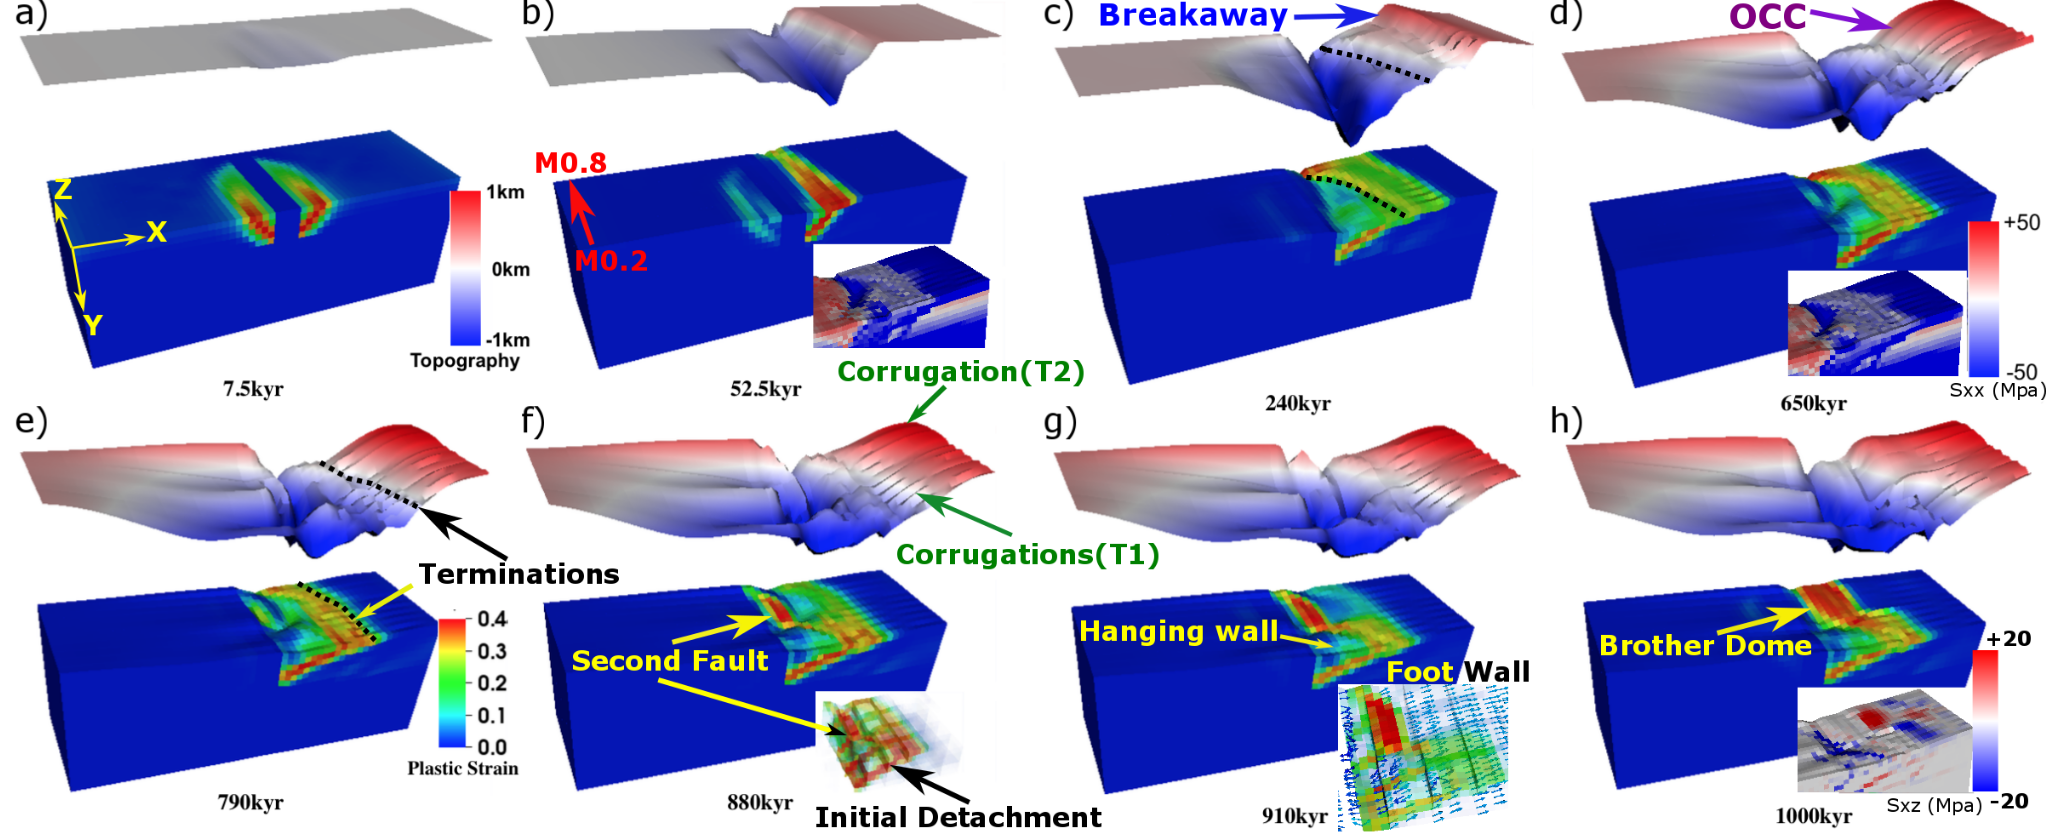
\includegraphics[width=1.0\textwidth]{fig_Results1_1.png}
  \caption{Reference model one: M linearly increases from 0.2 to 0.8 from front to back. The top layer is the topography of the model with five times vertical exaggeration. The green, yellow and red colors shown in the model domain are for Plastic strain. The number with kyr beneath is the time for the model with a unit of thousands of year. The two insets for 650kyr and 1000kyr is for shear stress $\sigma_{xz}$ (Sxz in the figure). The inset for 880kyr is for plastic strain. The inset for 910kyr shows both plastic strain and the velocity vector.} %\note[XT]{one thing to be noted is that the $dt=0.5yr$ in these series of 3D models, thus I divided the time step by two to get the time (kyr). This figure needs to be revised that the plastic strain scale is actually changing for different time, a way to revise it is to maintain a constant color scale or attach a color scale for each time. Also, it seems a little bit small and two rows is not as preferable as one row or one column to better express the concept of linear time series evolution.}}
 \label{fig_Results1_1}
\end{figure}   

\add[XT]{remember to add description for rotation: low M side begin to fault and bend and nuleate to high M side so that the faulting and bending is more or less simultaneous. Otherwise, it should be happening at different time. \\In addition, the lowest topo point along the ridge is oblique firstly in a xz direction (why is it happening) and later as the secondary fault evolves, another shear topo low (show in the inset of 1000kyr) in -xz direction take place due to movement (show in the inset of 910kyr) of the hanging wall at M$<0.5$ side is to the -x while at M$>0.5$ side its footwall is moving to +x thus create this shear low. Two shear low make a X shape and a huge ``corrugation'' on the left hand side of the ridge-axis }

As shown in Figure~\ref{fig_Results1_1}, at 7.5kyr, high angle ($\sim 60 \degree$ consistent with model parameter setup of frictional angle of 30$\degree$) normal faults (shown as high plastic strain shear bands) begin to form near the ridge axis because the thickness of the crust is thinnest at the ridge center according to model thermal structure. They first initiate at the front (lower M side) and then nucleate to the back (higher M side) because for each timestep, the tensional stress accummulates more at the lower M side and thus reach a yielding point earlier than higher M side. At 52.5kyr, the normal fault on the right hand side of the ridge axis continues to evolve while the one on the left becomes inactive. The choice of which fault will delvelop is a random event since the model setup is symmetrical across the ridge-axis. The timing difference of initiation of faulting along the ridge axis create a constant offset in X-axis direction of breakways that the breakaway at the lower M side extends further than that of the higher M side. However, this offset will not increase because the velocity for the breakaway to move away from the axis is only controlled by the far field extension rate, $V_{x}$.
%the fault displacement at the front side is larger than that of the back because M is lower at the front and more extension needed to be accommodated by the tectonic processes (i.e. normal faulting). \annote[XT]{Thus, the breakaway at the front extending further away from the ridge axis.}{I am not sure whether the breakaway extends further at lower M side because it should be the same. The breakaway at lower M side does extend further not because of fault slip rate difference but becauses of initiation time, at lower M side, fault begin earlier thus the breakaway begin to extend earlier and reach further, however, the rate of extending away from axis for the breakway should equal to the extension rate $V_{x}$. Thus the offset between breakaways of front and back remains constant} The termination of the detachment fault where footwall begins to be exhumed to the surface will extend further due of faster bending of the footwall at the lower M side. This will also result in a larger volume of exhumation at the lower M side than that of the higher M side. For our model that even when $M=0.2$, the detachment fault can still last for a long time, the exhumation rate has a upper limit of extension rate of $V_{x}$ in spite of a higher fault slip rate at lower M side.  

\begin{figure}[H]
  \centering
    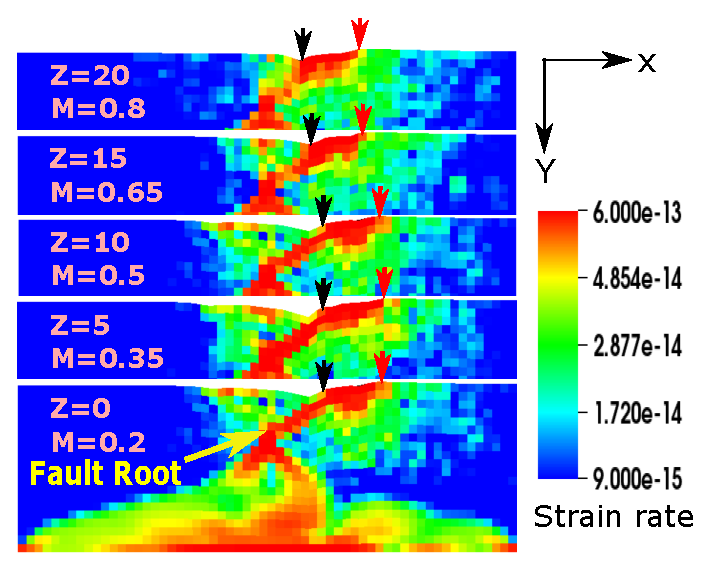
\includegraphics[width=0.6\textwidth]{fig_Results1_2.eps}
  \caption{Strain rate at 107.5kyr with five slices along ridge axis(Z axis).}
 \label{fig_Results1_2}
\end{figure}   

The location of the termination of the detachment fault where footwall begins to be exhumed to the surface varies along the ridge-axis (i.e. Z-axis). As shown in Figure~\ref{fig_Results1_2}, the highest strain rate regions can be interpreted as detachment fault interfaces. When M$<=0.5$, although the fault displacement should be higher for lower M, the rate of bending of the fault has a maximum value controlled by the far field extension rate, thus the faulting interfaces are similar. When M$>0.5$, the displacement as well as the amount of the bending of the fault decrease as M increases which help maintaining a higher angle fault and thus a nearer to the ridge-axis termination. However, this behavior is more or less compensated by the hanging wall being pushed away from the ridge-axis due to excessive diking (when M$>0.5$). In a unit time, the volume of the exhumation is also smaller for the higher M side.       

Corrugations are observed in the model since 240kyr. It will be further discussed in the discussion chapter. There are two contributing factors, for one, trans-extenstional stresses are created due to offset of the breakaway as well as the variation in fault displacements along the ridge axis; for the other, the variation of the position of the termination of the detachment fault might create anastomosing faults mentioned in \citep{Smith2014}.      

The secondary near axis high angle normal fault is another common observation of the models. As shown in Figure~\ref{fig_Results1_1}, at the ridge axis with M$>0.5$ (i.e. Z$>10$), the existing normal fault will be pushed away from the ridge-axis due to excessive diking, as its mechanism has been mentioned in the introduction chapter, another new near axis normal fault is created at around 650kyr. As it evolve, the initial detachment fault become inactive (the transparant view of plastic strain shown in the rigth corner inset of time 880kyr). This secondary fault creates another dome and its composition is more likely to be volcanic rather than ultramafic, however, as is evolve, if it can last long, lower crust and upper mantle material can be exhumed to the surface. The composition of the domes observed at Kane magamullions is similar to this mechanism that ultramafic Babel dome is on the West and crustal inside-corner high on the East.    

\subsubsection{Constant M along the ridge axis }

As shown in Figure~\ref{fig_Results1_3}, this constant M along the ridge-axis model create a median valley of $\sim 20km$ in width and $1\sim2km$ in depth which is similar to generally observation of Mid-Atlantic Ridges. The width and depth of the median valley is almost constant along the ridge-axis. The variation along the ridge-axis in breakaway and termination as well as the existence of corrugation mentioned in reference model one are not observed. 
\begin{figure}[H]
  \centering
    \includegraphics[width=1.0\textwidth]{fig_Results1_3.eps}
  \caption{Reference model two: constant M$=0.8$ along the ridge-axis (i.e. Z axis). Type two weakening.}
 \label{fig_Results1_3}
\end{figure}   

Based on the previous experience in pseudo-2D models or \citep{Lavier2000}, with higher characteristic fault displacement ($3dx \times Pls_{end}$), Type two weakening compared with Type one weakening, the frequency of normal faulting alternation, for M$>0.5$ cases, is higher. However, interesting enough, when comparing pseudo-2D and 3D models when they are using Type two weakening under case of M$=0.8$, even though the 3D Model has a larger $F_{slip_{c}}$ of 1km than that of pseudo-2D model of 0.5kmr, 3D model has a lower frequency of faulting alternation. 

\subsection{Tables of all the data points}


\begin{table}[H]
\begin{small}
\begin{center}
\begin{tabular}{||l|l||l|l||l|l||}
\hline
A & Alternating Fault & C & Corrugation & SL & Shear Topography Low \\
\hline
NA& Not Alternating & SF & Secondary Fault on one side & CB & Cut Back   \\
\hline
DD &  Double Dome  & AM    & Atlantis Massif &  &   \\
\hline
\end{tabular}
\end{center}
\end{small}
\caption{Model behaviors in short.}
\end{table}


\begin{table}[H]
\begin{small}
\begin{center}
\begin{tabular}{|l|p{3.5cm}|p{3.5cm}|p{3.5cm}|}
\hline
\diagbox[width=12em]{Weakening type}{M range}&
M28&M57&M58\\
\hline
Type one &NA; C; SL; SF$_{1500kyr}$; DD    &NA; C; SF$_{1380kyr}$; CB$_{330kyr}$; AM(opposite z)     &    \\
\hline
Type two &    &     &    \\
\hline
\end{tabular}
\end{center}
\end{small}
\caption{Linear functional form.}
\end{table}

\begin{center}
\begin{table}[H]
\begin{small}
\begin{tabular}{|l|p{3.5cm}|p{3.5cm}|p{3.5cm}|}
\hline
\diagbox[width=12em]{Weakening type}{M range}&
M28&M57&M58\\
\hline
Type one & NA; C; SL; SF$_{995kyr}$ & NA; C; SL; SF$_{760kyr;1320kyr}$; CB$_{520kyr}$; AM & NA; C; SL; CB$_{510kyr}$; SF$_{760kyr;1140kyr;1990kyr}$   \\
\hline
Type two &    &NA; C; SL; SF$_{680kyr}$; CB$_{905kyr}$     & A$_{450kyr;600kyr}$; C(only at low M); CB$_{990kyr}$   \\
\hline
\end{tabular}
\end{small}
\caption{Sinusoidal functional form.}
\end{table}
\end{center}

\begin{table}[H]
\begin{small}
\begin{center}
\begin{tabular}{|l|p{3.5cm}|p{3.5cm}|p{3.5cm}|}
\hline
\diagbox[width=12em]{Weakening type}{M range}&
M28&M57&M58\\
\hline
Type one & NA; C; SL; CB$_{205kyr;330kyr;1025kyr}$   &      & NA; C$_{1770kyr}$(due to shear with dif wave length); SF$_{860kyr}$(high M); SF$_{1190kyr}$(low M)(Dog Bone); SF$_{1690kyr}$    \\
\hline
Type two &    & NA; C; SF$_{435kyr;1060kyr}$; CB$_{585kyr}$; CB$_{735kyr}$; CB$_{910kyr}$; CB$_{970kyr}$    & A$_{550kyr;920kyr}$; C; CB$_{400kyr}$    \\
\hline
\end{tabular}
\end{center}
\end{small}
\caption{Square root functional form.}
\end{table}

\subsection{Fault Alternation}
The fault alternation behavior observed in pseudo-2D models in cases M$>0.5$ is much more complicated in 3D models. The results shows that only Type two weakening with M58 will result in a alternating faulting pattern. \add[XT]{integrate the area of M$>0.5$ with respect to Z to see if there is any quantatative analysis available.}

\subsection{Variation of the range of M}

\subsection{Variation of the functional form}

\subsection{Influence of weakening rate}

\subsection{Summary of Findings}
